\documentclass{beamer}

%\documentclass{beamer}
\usepackage[utf8]{inputenc}
\usepackage{graphicx}

%% Configure Beamer

% Bblue for emphasising text
\newcommand{\bblue}[1]{{\usebeamercolor[fg]{frametitle}{#1}}}


% Enables logo
\setbeamertemplate{background}
{
\includegraphics[width=\paperwidth,height=\paperheight,keepaspectratio]{gu-background.pdf}}
%{
\includegraphics[width=\paperwidth,height=\paperheight,keepaspectratio]{gu-background-16_9.pdf}} % for 16:9


% Makes hyperlinks beamer blue
%\definecolor{links}{HTML}{2A1B81}
\definecolor{links}{cmyk}{0.72,0.72,0,0.3}
\hypersetup{colorlinks,linkcolor=,urlcolor=links,citecolor=links}

\usepackage{graphicx}
\graphicspath{ {./pic/} }

% Add slide counter at the bottom
\setbeamertemplate{footline}[frame number]

\title{Hands-on
	\\ Robot Operating System (ROS)
	\\ programming robots and language technology}
\author{Aram Karimi}
\institute{LT2318 H21 Artificial Intelligence: Cognitive Systems}
\date{November 22th, 2020}

	




\begin{document}
	\frame{\titlepage}
	\begin{frame}
	Outline
		\begin{itemize}
			\item Intelligent Agent
			\item Agents and environments
			\item Robot Operating System(ROS)
			\begin{itemize}
				\item A “Meta” Operating System.
				\item Nodes
				\item Message passing
				\item Multiple language support
			\end{itemize}
			\item Hands-on Tutorial
			\begin{itemize}
				\item Ros Installation
				\item Connect to kinect
				\item Keras in ROS
			\end{itemize}
		\end{itemize}
	\end{frame}

	\begin{frame}
		\begin{figure}[l]
			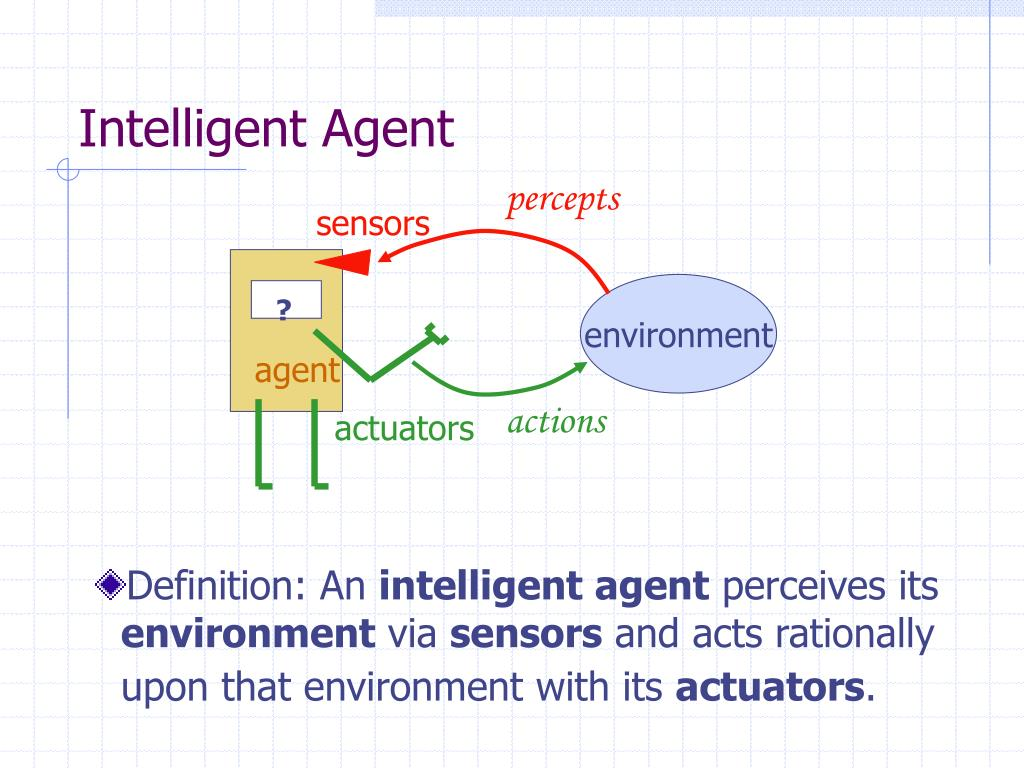
\includegraphics[scale=0.35]{intelligent-agent-l.jpg}
		\end{figure}
	\end{frame}
	
	\begin{frame}
		Characteristics of intelligent agents:
		\begin{itemize}
			\item They have some level of autonomy that allows them to perform certain tasks on their own.
			\item They have a learning ability that enables them to learn even as tasks are carried out.
			\item They can interact with other entities such as agents, humans, and systems.
			\item New rules can be accommodated by intelligent agents incrementally.
			\item They exhibit goal-oriented habits.
			\item They are knowledge-based. They use knowledge regarding communications, processes, and entities.
		\end{itemize}
		
	\end{frame}
	
	\begin{frame}
		\textbf{Agents include humans, robots, softbots, thermostats, etc.}
		The agent function maps from percept histories to actions:
		\begin{equation}
			f \colon P^{*} \to A .
		\end{equation}
		The agent program runs on the physical architecture to produce	$f$ \\
		\textbf{How do we know if this is a good agent function?} \\
		\begin{itemize}
			\item What is the best function?
			\item Is there one? 
			\item Who decides this? 
		\end{itemize}		
	\end{frame}
	\begin{frame}
		Vacuum-cleaner world
		\begin{figure}
			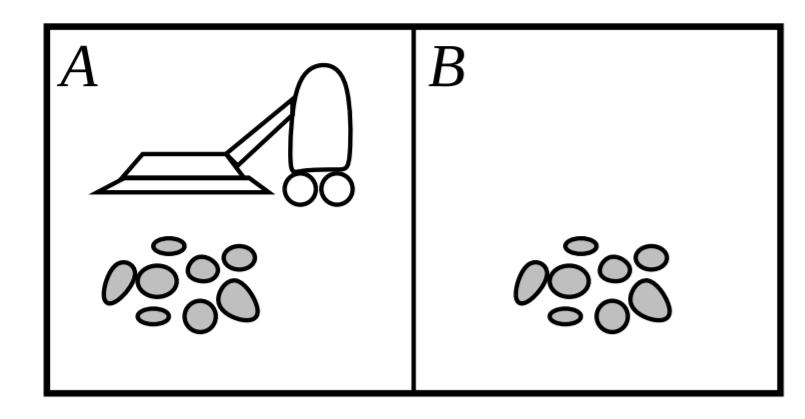
\includegraphics[scale=0.25]{vc.jpeg}
		\end{figure}
		Percepts: location and contents, e.g., $[A, Dirty]$ \\
		Actions: $Left, Right, Suck, NoOp$ \\
		\textbf{A simple agent function is:} \\
		If the current square is dirty, then suck; \\
		otherwise, move to the other square.
	\end{frame}

	\begin{frame}
		Rationality:
		\textbf{A rational agent chooses any action that}
		\begin{itemize}
			\item maximizes the expected value of the performance measure
			\item given the percept sequence to date
		\end{itemize}
		$Rational \neq omniscient$
		\begin{itemize}
			\item  percepts may not supply all relevant information
		\end{itemize}
		$Rational \neq clairvoyant$
		\begin{itemize}
			\item  action outcomes may not be as expected
		\end{itemize}
		$Rational \neq successful$
		\begin{itemize}
			\item $Rational \implies exploration, learning, autonomy$
		\end{itemize}
	\end{frame}
	\begin{frame}
		Agent types \\
		Four basic types in order of increasing generality:\\
		\begin{itemize}
			\item simple reflex agents
			\item reflex agents with state
			\item goal-based agents
			\item utility-based agents
		\end{itemize}
	All these can be turned into learning agents
	\end{frame}

	\begin{frame}
	\centering
		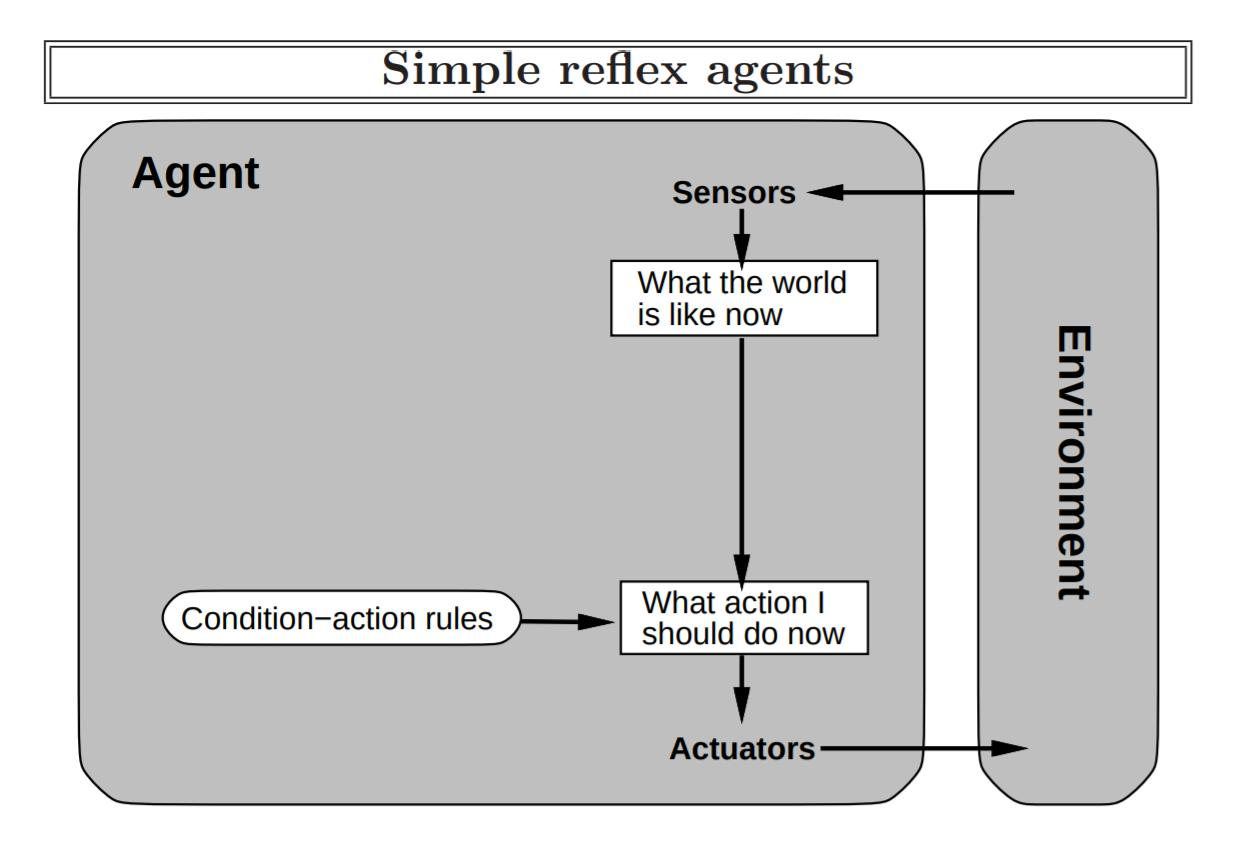
\includegraphics[scale=0.21]{a1.jpeg}
	\end{frame}

	\begin{frame}
		\centering
		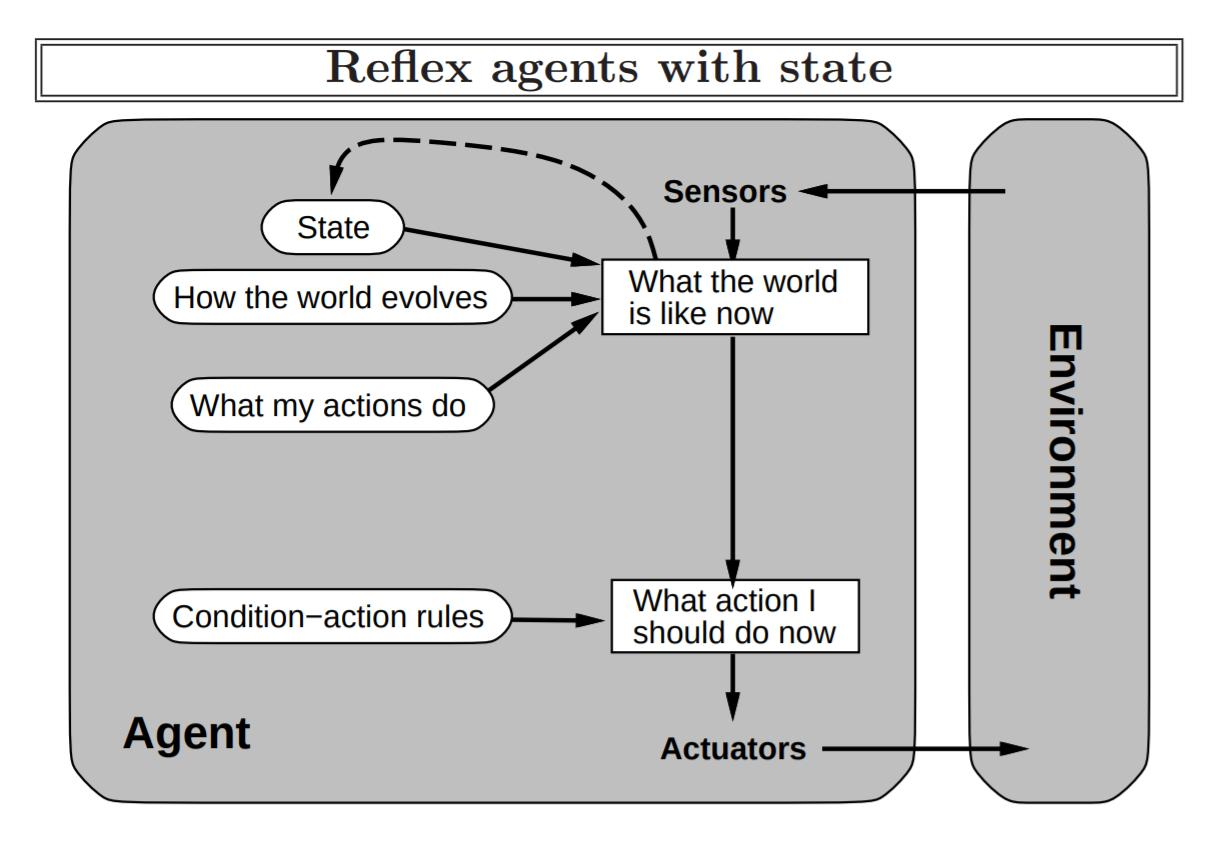
\includegraphics[scale=0.21]{a2.jpeg}
	\end{frame}

	\begin{frame}
		\centering
		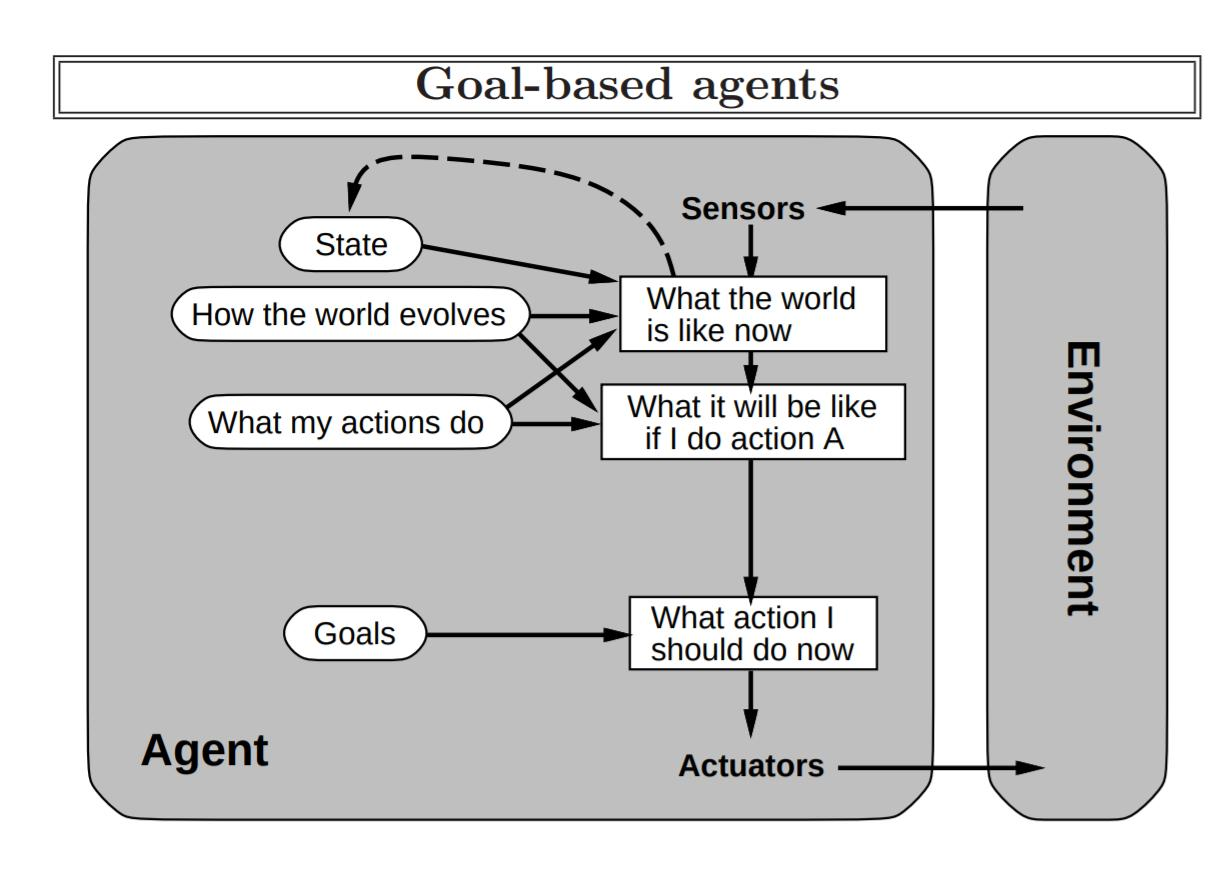
\includegraphics[scale=0.21]{a3.jpeg}
	\end{frame}

	\begin{frame}
		\centering
		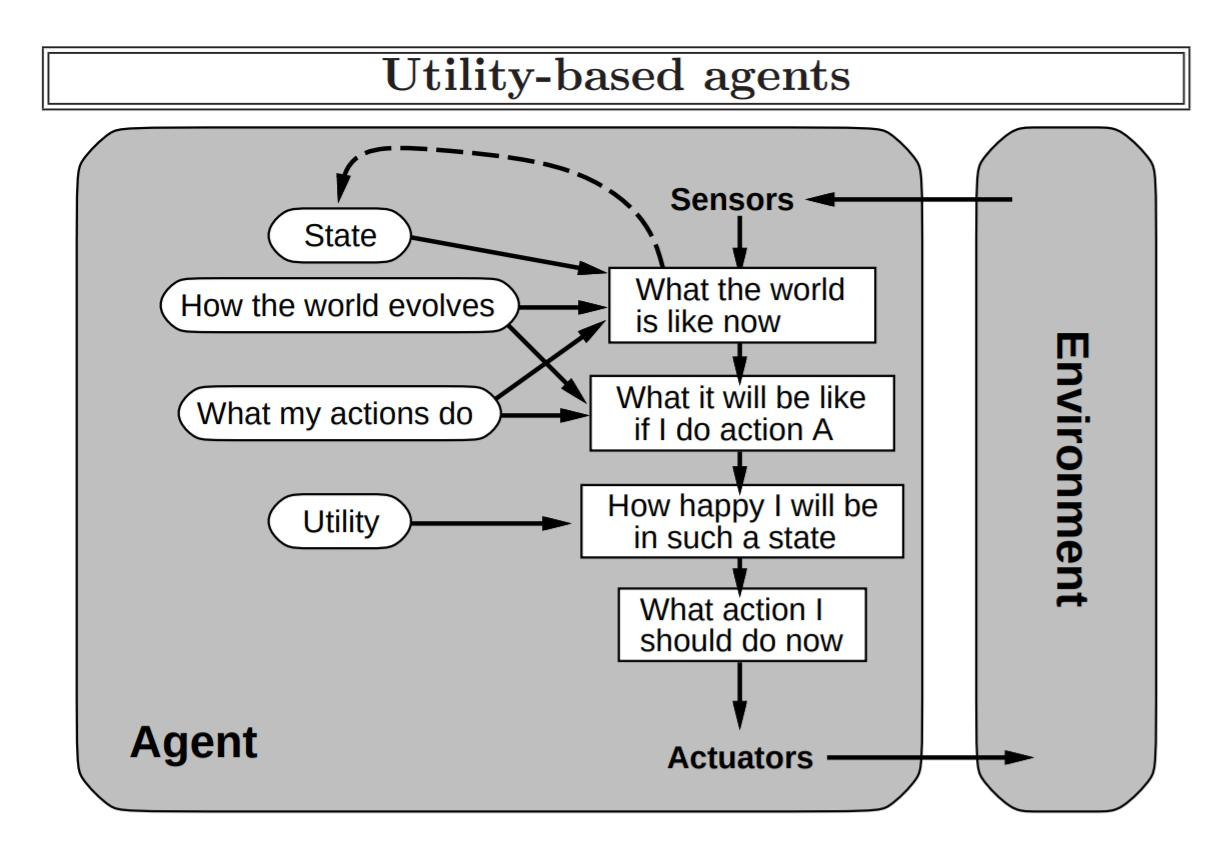
\includegraphics[scale=0.21]{a4.jpeg}
	\end{frame}

	\begin{frame}
		\centering
		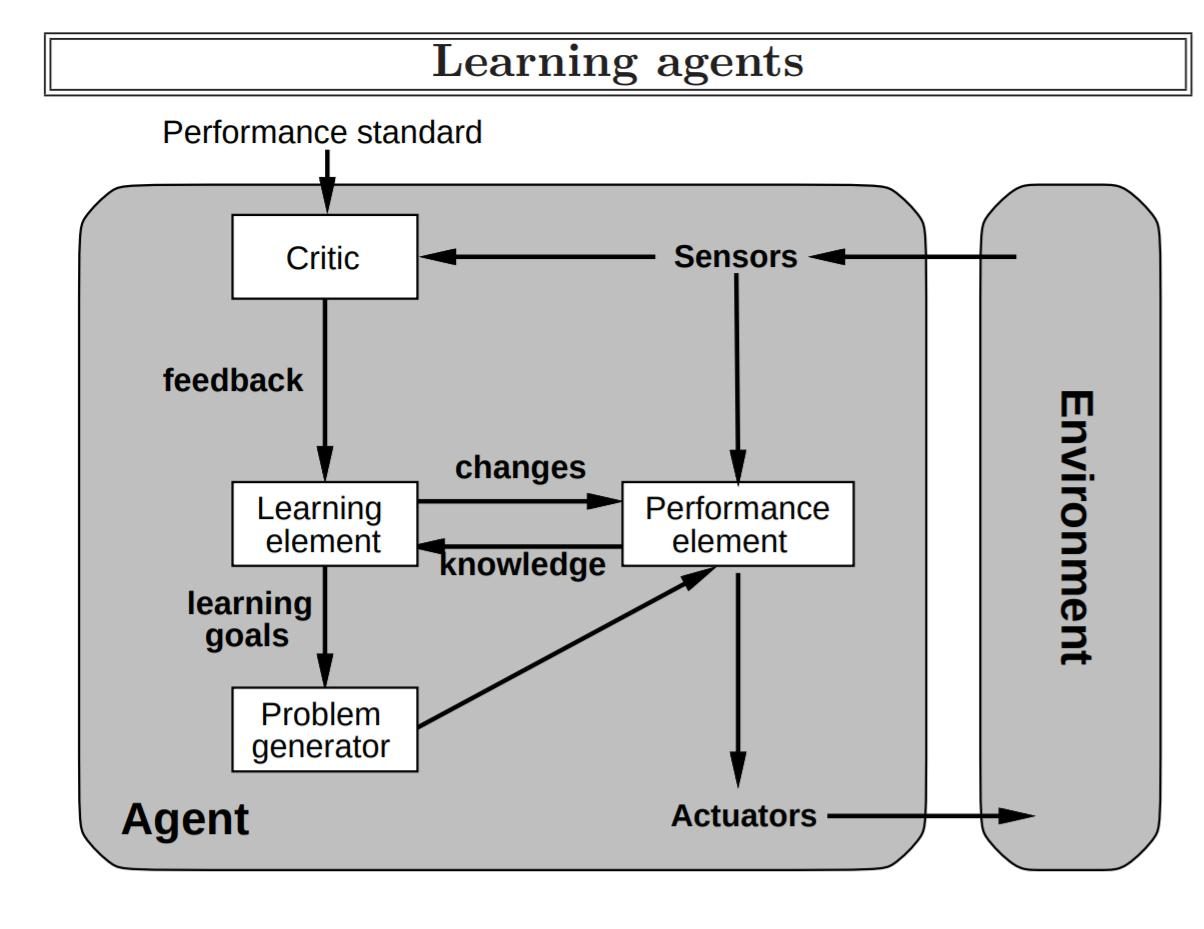
\includegraphics[scale=0.21]{a6.jpeg}
	\end{frame}

	\begin{frame}
		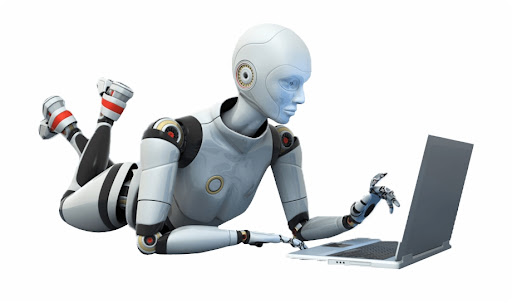
\includegraphics[scale=0.54]{ed.jpg}
	\end{frame}

	\begin{frame}
		What is ROS(Robotic Operating System)?
		\begin{itemize}
			\item It is not a Operating System (OS)
			\item It is not an Application Programming Interface (API)
			\item It is not a simple framework
		\end{itemize}
		\textbf{ROS is a middleware for robotic programming, specifically designed for complex applications}
		\begin{itemize}
			\item ROS is a platform for robot software.
			\item Hardware abstraction
			\item Message passing between nodes
			\item Sophisticated build environment
			\item Advance open-source robotics
			\item Debugging and Visualization Tools
		\end{itemize}
	\end{frame}
	\begin{frame}
	\textbf{ROS as a framework } \\
		The ROS framework is component oriented. \\
		Each component is called a node. Nodes communicate using topics or services.
		\begin{itemize}
			\item topics represents data-flow. For instance: camera images, robot configuration or position can be model as topics. Topics values are often published regularly to keep the whole system up-to-date.
			\item services represents queries which are sent asynchroneously, and usually at a low frame-rate. Slow components such as motion planning nodes for instance usually provide services.
		\end{itemize}
	\end{frame}
	\begin{frame}
	The ROS framework is a graph
		\begin{itemize}
			\item Each node can listen or publish on a topic
			\item Each node can call or provide one or more services.
			\item Each node can also set or get one or more parameters. Some are public	and can be modified by other nodes. The other are private and are defined at startup only.
		\end{itemize}
		Packages
		\begin{itemize}
			\item ROS software is organized into packages
			\item Each package contains some combination of	code, data, and documentation
		\end{itemize}
	\end{frame}
	\begin{frame}
		ROS Architecture: Basics
		\begin{figure}
			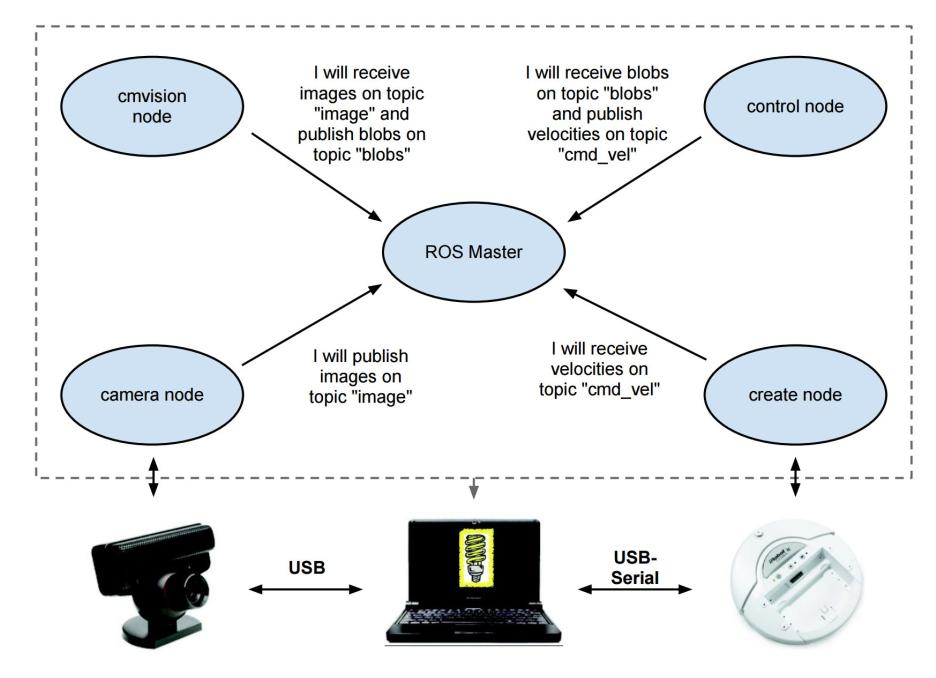
\includegraphics[scale=0.28]{ros_arc.jpeg}
		\end{figure}
	\end{frame}

	\begin{frame}
		Why ROS? \\
		\begin{itemize}
			\item Avoid complexity of a big software.
			\item Abstraction for specific robot hardware.
			\item Sequential programming on asynchronous environment.
			\item Setting up the Robot takes too much time
			\item Programs can be run on multiple computers and communicate over the network.
			\item Multi-language support
			\item Free and open-source
		\end{itemize}
	\end{frame}

	\begin{frame}
		Configuring the ROS environment
		\begin{itemize}
			\item You need Ubuntu (Install Virtualbox if you don't have Ubuntu)
			\item  Programming knowledge (Python, C++)
			\item Robot simulation / any robot compatible with ROS:
			\begin{itemize}
				\item http://wiki.ros.org/Robots
			\end{itemize}
			\item Robotics by nature is multi-disciplinary:	Some knowledge from other fields is required.
			\item Use open-source projects
		\end{itemize}
	\end{frame}
	\begin{frame}
	\centering
		\huge Live Coding!
	\end{frame}
	\begin{frame}
		References
	\end{frame}
\end{document}
